
El algoritmo de Cristian es un método para la sincronización de reloj que se
puede utilizar en muchos campos de la informática distributiva, los procesos
del cliente utilizan para sincronizar la hora con un servidor de
tiempo pero se utiliza principalmente en intranets de baja latencia.
El objetivo de este algoritmo es que es que todas las demás máquinas permanezcan sincronizadas con la \textit{maquina maestra}.
\begin{figure}[H]
  \centering
  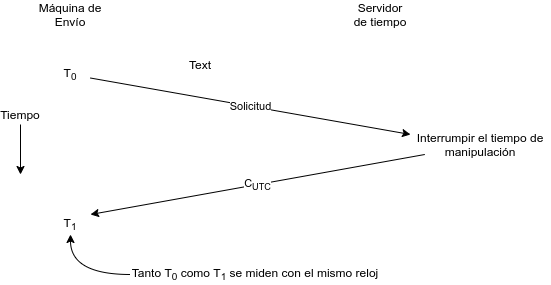
\includegraphics[width=10cm]{ac}
  \caption{Obtener la hora actual de un servidor.}\label{fig:4}
\end{figure}.

\begin{listing}[H]
\inputminted[
  frame=lines,
  framesep=2mm,
  baselinestretch=1.2,
  bgcolor=LightGray,
  fontsize=\scriptsize,
  linenos,
  firstline=7,
  %lastline=49
  ]{python}{../cristian/Workbench.py}
\caption{Workbench.py de algoritmo Cristian}
\label{lst:4}
\end{listing}

Inicializamos el maestro, hacemos uso de los sockets
\mintinline{shell}{tcp://localhost} junto con  puertos
$10000$, $10001$ y $10003$ para los Slaves y los registramos en el maestro
para después sincronizarlos.

\begin{listing}[H]
\inputminted[
  frame=lines,
  framesep=2mm,
  baselinestretch=1.2,
  bgcolor=LightGray,
  fontsize=\scriptsize,
  linenos,
  firstline=14,
  lastline=50
  ]{python}{../cristian/Server.py}
\caption{Server.py del algoritmo Cristian}
\label{lst:5}
\end{listing}
\clearpage

La clase \textsc{Cliente} se encarga de la implementación de los Slaves,
la cuál inicializa y, mediante una respuesta del Master (\textsc{Clase Server})
se sincroniza con ellos mediante el uso de la siguiente fórmula implementada
en el método \mintinline{shell}{obtener_tiempo} de la clase Server Código~\ref{lst:5}:
\begin{equation}
  \label{eq:1}
  \frac{T_{client}= T_{server}+(T_{1}-T_{o})}{2}
\end{equation}

Donde:

\begin{itemize}
  \item $T_{client}$ refiere a la hora del reloj sincronizado.
  \item $T_{server}$ refiere a la hora del reloj devuelta por el servidor.
  \item $T_{0}$ refiere  a la hora a la que el proceso del cliente envió la
        solicitud.
  \item $T_{1}$  a la hora a la que el proceso del cliente envió la solicitud,
\end{itemize}

\begin{listing}[H]
\inputminted[
  frame=lines,
  framesep=2mm,
  baselinestretch=1.2,
  bgcolor=LightGray,
  fontsize=\scriptsize,
  linenos,
  firstline=11,
  % lastline=50
  ]{python}{../cristian/Client.py}
\caption{Client.py del algoritmo Cristian}
\label{lst:6}
\end{listing}


\begin{figure}[H]
  \centering
  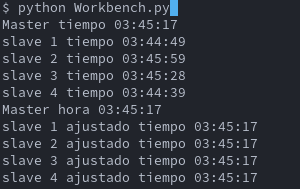
\includegraphics[width=8cm]{ex_c}
  \caption{Ejecucuión de Workbench.py}\label{fig:5}
\end{figure}
